\subsection{AFFINE WEYL GROUP AND COMPLETED DYNKIN GRAPH}

Let R be an irreducible reduced root system and let \((\mathbf{X}, f)\) be its Dynkin graph. We are going to define another normed graph \((\tilde{\mathbf{X}}, \tilde{f})\) that we shall call the completed Dynkin graph of R. The set \(\tilde{I}\) of vertices of \(\tilde{X}\) consists of the set I of vertices of X and a vertex denoted by 0, not belonging to I. To define \(\tilde{f}\) , choose a basis \(B = (\alpha_{i})_{i \in I}\) of R and a scalar product \((x|y)\) invariant under W(R). Let \(\alpha_{0}\) be the negative of the highest root for the order defined by B. Two distinct vertices \(i, j \in \tilde{I}\) are linked if and only if \((\alpha_{i}|\alpha_{j}) \neq 0\) and we then put

\[
\tilde {f} (i, j) = \frac {\left(\alpha_ {i} \mid \alpha_ {i}\right)}{\left(\alpha_ {j} \mid \alpha_ {j}\right)}.
\]

It is immediate that the graph \(\tilde{X}\) and the map \(\tilde{f}\) thus defined do not depend on the choice of B or the scalar product.

If the rank \(l\) of \(R\) is equal to 1, then \(I = \{i\}\) and \(\alpha_0 = -\alpha_1\) ; hence \(\tilde{f}(0, i) = 1\) . If \(l \geqslant 2\) , \(\alpha_0\) is not proportional to any of the \(\alpha_i\) and \((\alpha_0|\alpha_i)\) is \(\leqslant 0\) (§ 1. no. 8. Prop. 25). For any pair \((i,j)\) of distinct elements of \(\tilde{I}\) , the only possibilities are those denoted by 1), 2), 3), 4) in the preceding number (putting, for example, \(n_{0i} = n(\alpha_0, \alpha_i)\) and \(m_{0i} = \text{order of } s_{\alpha_0}s_{\alpha_i}\) for all \(i \in I\) ).

In the case \(l \geqslant 2\) , the completed Dynkin graph is represented by a diagram with the same conventions as in the preceding number, sometimes indicating by dotted lines the bonds joining the vertex 0 to the other vertices. We remark that the inequality sign \textgreater{} on such a bond, if it exists, is always directed towards the vertex distinct from 0, since \(\alpha_{0}\) is a longest root ( \(\S\) 1, no. 8, Prop. 25). The graph \((\mathbf{X}, f)\) is the subgraph obtained from \((\tilde{\mathbf{X}}, f)\) by deleting the vertex 0.

The action of A(R) on (X. f) extends to an action on \((\tilde{\mathbf{X}}.\tilde{f})\) , leaving 0 fixed, and W(R) acts trivially on \((\tilde{\mathbf{X}}.\tilde{f})\) .

We retain the notations of § 2. Prop. 5 of § 2, no. 2, together with Th. 1 of Chap. V, § 3, no. 2, shows that the Coxeter graph \(\Sigma\) of the affine Weyl group \(W_{a}(R)\) can be obtained from \((\tilde{X},\tilde{f})\) by the same rules by which the Coxeter graph of \(W(R)\) is obtained from \((X,f)\) . On the other hand, let G be the normaliser of \(W_{a}(R)\) (§ 2, no. 3). To any \(g\in G\) corresponds an automorphism \(\varphi(g)\) of \(\Sigma\) and \(\varphi(g)=\mathrm{Id}\) if \(g\in W_{a}(R)\) . Conversely, given an automorphism \(\lambda\) of \(\Sigma\) there is, by Prop. 11 of Chap. V, § 4, no. 9, a unique element \(g=\psi(\lambda)\) preserving a given alcove C and such that \(\varphi(g)=\lambda\) . Since G is the semi-direct product of the subgroup \(G_{C}\) of elements preserving C and \(W_{a}(R)\) (§ 2, no. 3), we deduce that \(\varphi\) defines by passage to the quotient an isomorphism from \(G/W_{a}\) (or from \(G_{C}\) ) to \(\operatorname{Aut}(\Sigma)\) . It is immediate that the composite of this isomorphism with the canonical map from A(R)/W(R) to G/ \(W_{a}\) coincides with the homomorphism from A(R)/W(R) to \(\operatorname{Aut}(\Sigma)\) induced by the homomorphism from A(R)/W(R) to \(\operatorname{Aut}(\tilde{X},\tilde{f})\) defined above. By § 2, no. 3, the group \(\operatorname{Aut}(\Sigma)\) is isomorphic to the semi-direct product of

\(A(R)/W(R)\) by \(P(R')/Q(R')\) , and \(P(R')/Q(R')\) is isomorphic to the group \(I_{C'} = G_{C'} \cap W_{a}'\) (with the notation of § 2. no. 3): the element of \(\text{Aut}(\Sigma)\) corresponding to the element \(\gamma_{i}\) of \(I_{C}\) transforms the vertex 0 to the vertex i of \(\Sigma\) .

Remark. It can be shown that the canonical map

\[
\operatorname{Aut} (\tilde {X}, \tilde {f}) \rightarrow \operatorname{Aut} (\Sigma)
\]

is an isomorphism.

THEOREM 4. Let (W.S) be an irreducible Coxeter system with S finite. The associated quadratic form (Chap. V. § 4, no. 1) is positive and degenerate if and only if the Coxeter graph of (W.S) is isomorphic to one of the following:

\pandocbounded{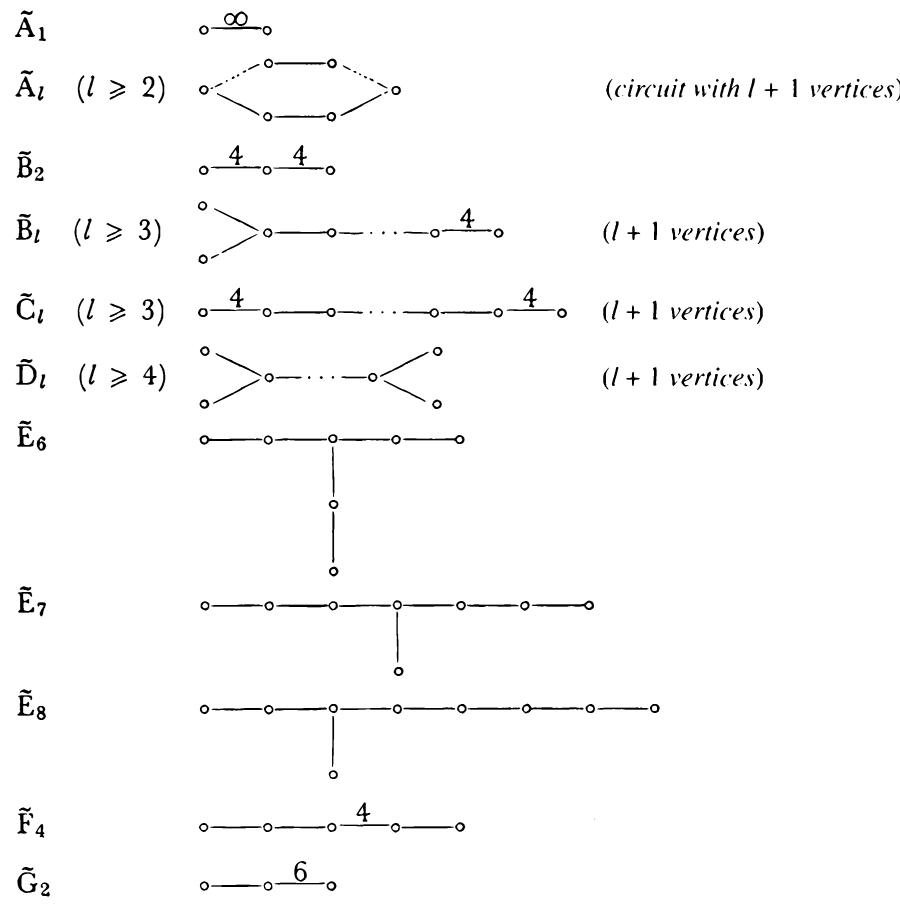
\includegraphics[keepaspectratio]{images/part002_b5f8d83f.jpg}}

No two of these Coxeter graphs are isomorphic.

By Chap. V. § 4, no. 9 and Prop. 8 of § 2, no. 5, the Coxeter systems whose quadratic form is positive and degenerate are those which correspond to the affine Weyl groups of irreducible reduced root systems. The theorem therefore follows from the determination of the completed Dynkin graphs made in nos. 5 to 13 below.

